%%%%%%%%%%%%%%%%%%%%%%%%%%%%%%%%%%%%%%%%%%%%%%%%%%%%%%%%%%
\chapter{FLOWPAK: Flow-based Ornamental Element Packing}
%%%%%%%%%%%%%%%%%%%%%%%%%%%%%%%%%%%%%%%%%%%%%%%%%%%%%%%%%%

\mynote{Chapter title too long --> https://tex.stackexchange.com/questions/335346/addcontentslinetoc-with-a-linebreak-or-newline-for-the-toc}


%%%%%%%%%%%%%%%%%%%%%%%%%%%%%%%%%%%%%%%%%%%%%%%%%%%%%%%%%%
\section{Introduction}
%%%%%%%%%%%%%%%%%%%%%%%%%%%%%%%%%%%%%%%%%%%%%%%%%%%%%%%%%%

\begin{figure}[ht] %%% ELEMENT IMAGE
\centering
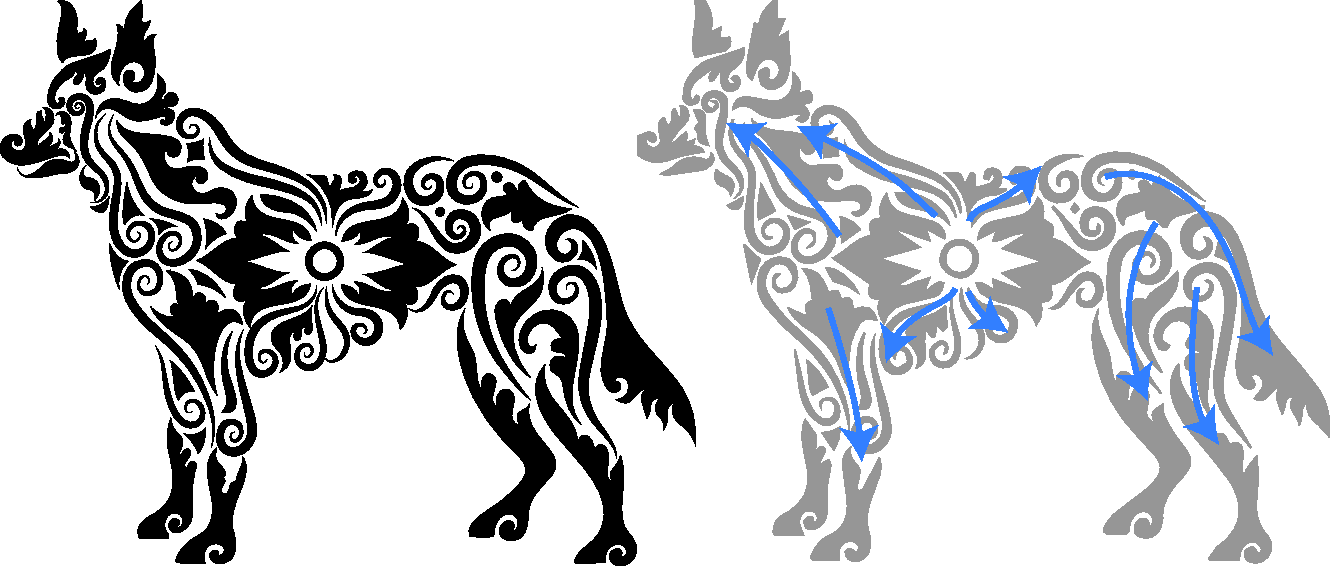
\includegraphics[width=0.6\textwidth]{figures/flowpak/dog_ornament_flow.pdf}
\vspace*{-8pt}
\caption{
  \label{dog_flow}
  An example of flow visual style, 
  including a visualization of the flow directions
of elements (by ComicVector703 on Shutterstock).
}
\end{figure}

FLOWPAK~\cite{Saputra2017} is a technique for filling a container 
region with elements that are deformed 
to communicate a sense of directionality or flow.
Elements can be oriented in the local direction 
of flow, but can also be deformed to capture changes in flow direction.
Flow adds visual interest to a composition,
engaging the viewer by providing a sense of progression and
movement through elements.
A hand-drawn dog example in Fig.~\ref{dog_flow} shows many elements that appear to flow
outward from the flower in the centre of the torso, and then
up the neck and down into the legs.
Although there has been a moderate amount of past research on
the generation of packings or mosaics,
this past work is not appropriate for creating flow-like
designs similar to the dog example.


%%%%%%%%%%%%%%%%%%%%%%%%%%%%%%%%%%%%%%%%%%%%%%%%%%%%%%%%%%
\section{Previous Work}
%%%%%%%%%%%%%%%%%%%%%%%%%%%%%%%%%%%%%%%%%%%%%%%%%%%%%%%%%%


%%%%%%%%%%%%%%%%%%%%%%%%%%%%%%%%%%%%%%%%%%%%%%%%%%%%%%%%%%
\section{Problem Formulation}
%%%%%%%%%%%%%%%%%%%%%%%%%%%%%%%%%%%%%%%%%%%%%%%%%%%%%%%%%%


%%%%%%%%%%%%%%%%%%%%%%%%%%%%%%%%%%%%%%%%%%%%%%%%%%%%%%%%%%
\section{Approach}
%%%%%%%%%%%%%%%%%%%%%%%%%%%%%%%%%%%%%%%%%%%%%%%%%%%%%%%%%%


\begin{figure}
\centering
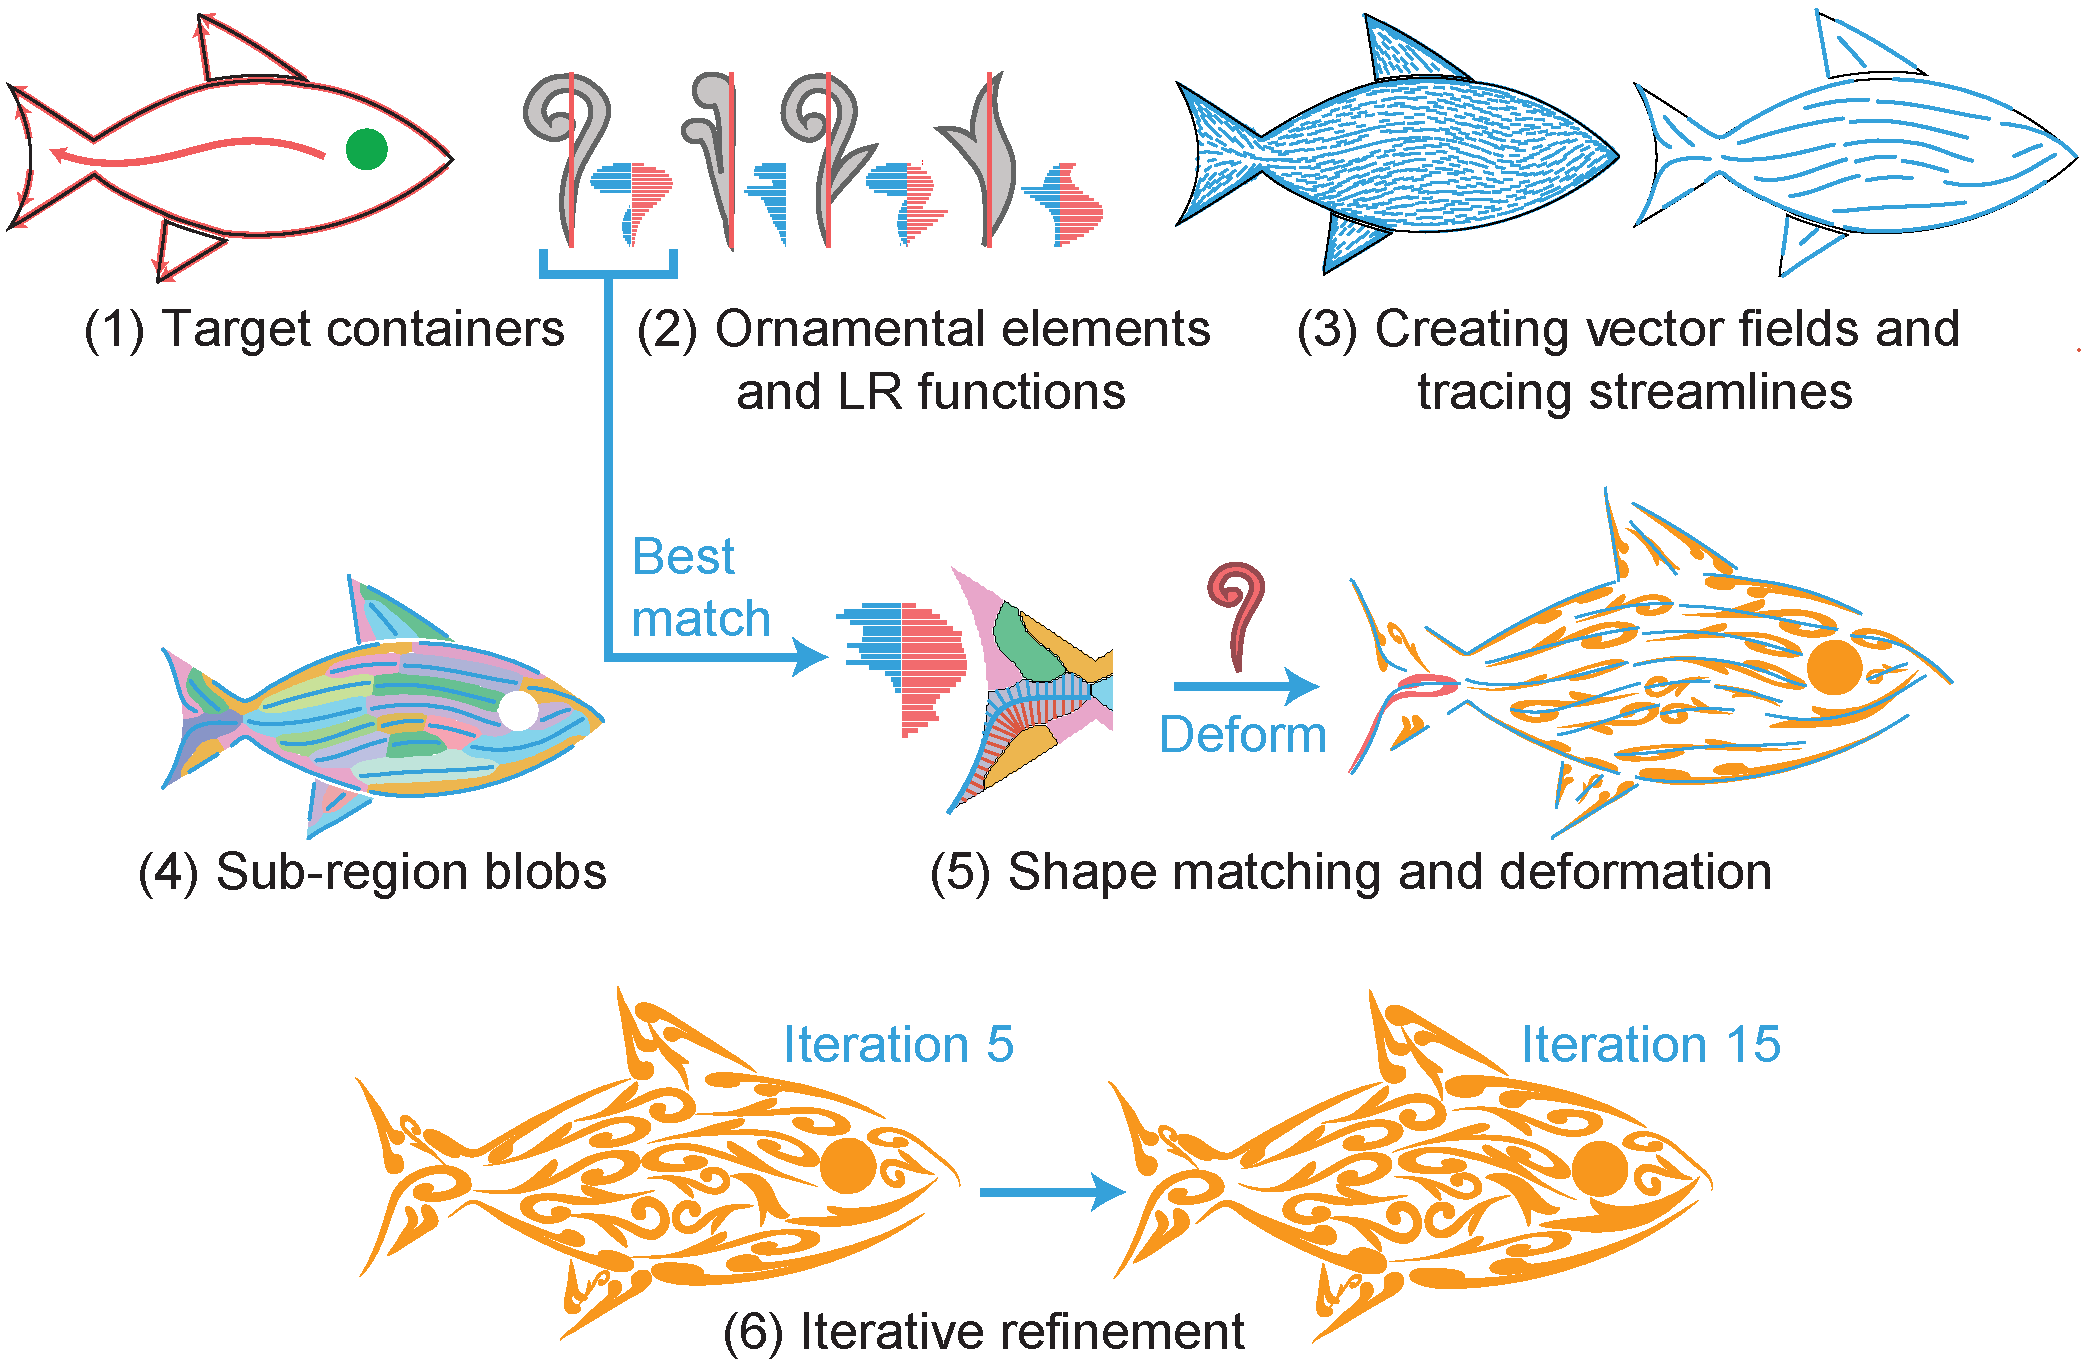
\includegraphics[width=1.0\textwidth]{figures/flowpak/pipeline.pdf} 
\caption{\label{fig_flowpak_pipeline} 
FLOWPAK pipeline. \mynote{Need rearrange}.}
\end{figure}

%%%%%%%%%%%%%%%%%%%%%%%%%%%%%%%%%%%%%%%%%%%%%%%%%%%%%%%%%%
\subsection{Target Containers}
%%%%%%%%%%%%%%%%%%%%%%%%%%%%%%%%%%%%%%%%%%%%%%%%%%%%%%%%%%


%%%%%%%%%%%%%%%%%%%%%%%%%%%%%%%%%%%%%%%%%%%%%%%%%%%%%%%%%%
\subsection{Ornamental elements and LR functions}
%%%%%%%%%%%%%%%%%%%%%%%%%%%%%%%%%%%%%%%%%%%%%%%%%%%%%%%%%%

\begin{figure}
\centering
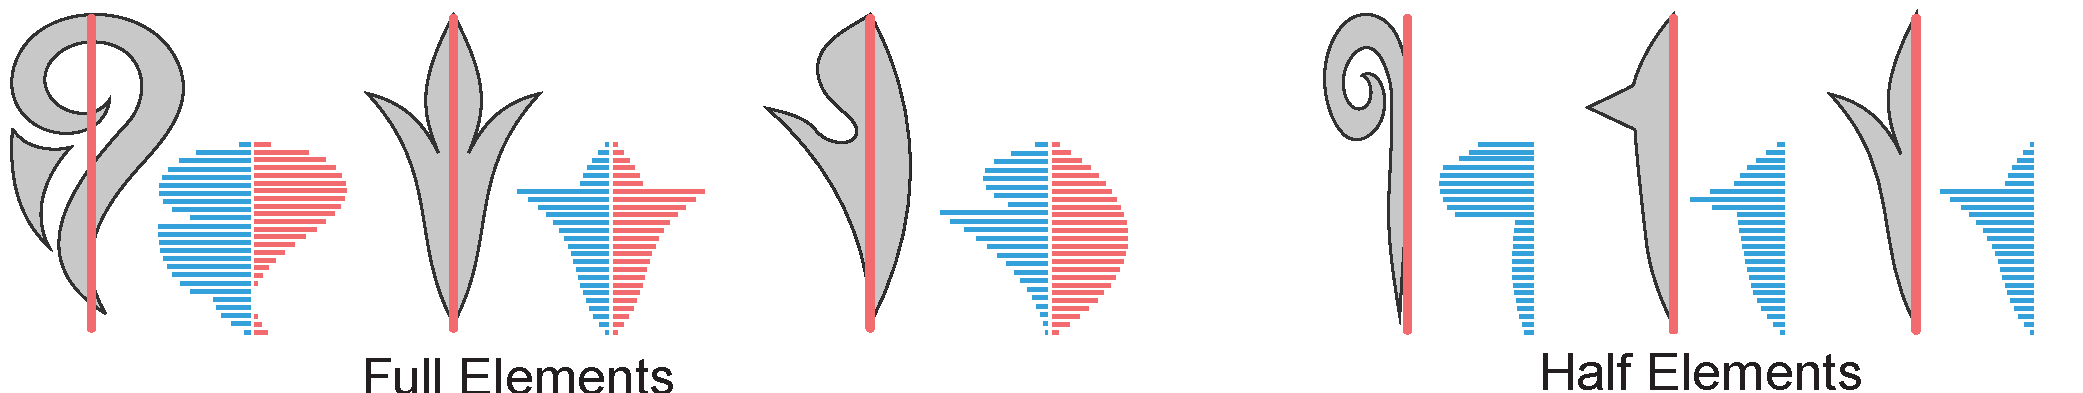
\includegraphics[width=1.0\textwidth]{figures/flowpak/ornaments.pdf}
\caption{\label{ornamental_shapes_fig}
Ornamental elements and their LR functions. Full elements have non-empty
left and right sides, while half elements have only one non-empty side. 
We normalize the LR functions to a unit square.}
\end{figure}

%%%%%%%%%%%%%%%%%%%%%%%%%%%%%%%%%%%%%%%%%%%%%%%%%%%%%%%%%%
\subsection{Creating Vector Fields and Tracing Streamlines}
%%%%%%%%%%%%%%%%%%%%%%%%%%%%%%%%%%%%%%%%%%%%%%%%%%%%%%%%%%

\begin{figure}
\centering
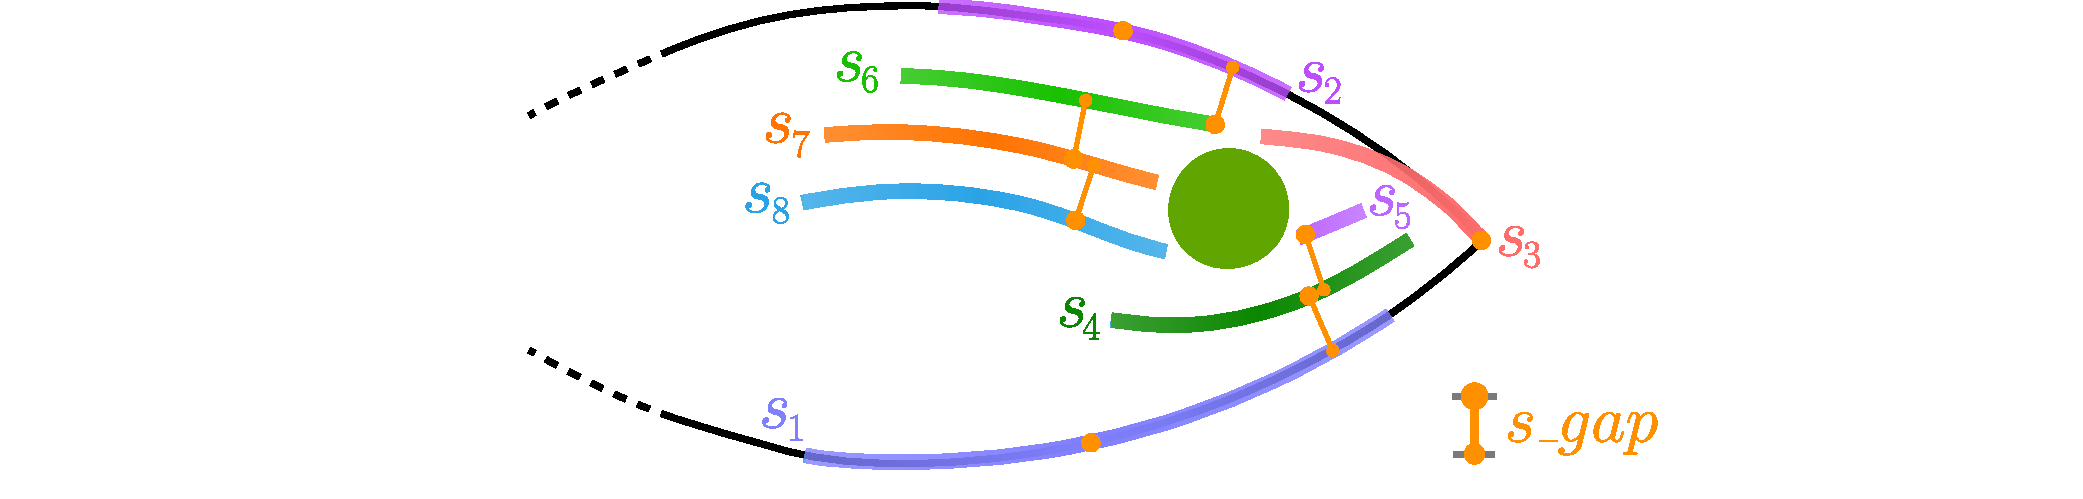
\includegraphics[width=1.0\textwidth]{figures/flowpak/streamline_tracing.pdf}
\caption{\label{streamline_tracing}
The streamline tracing process. The first streamline $s_1$ always begins
on a directional guide or the container boundary.  Subsequent streamlines begin
on the container boundary, a directional guide, or at a point that is 
$d\_gap$ away from a previous streamline.}
\end{figure}

%%%%%%%%%%%%%%%%%%%%%%%%%%%%%%%%%%%%%%%%%%%%%%%%%%%%%%%%%%
\subsection{sub-region blobs}
%%%%%%%%%%%%%%%%%%%%%%%%%%%%%%%%%%%%%%%%%%%%%%%%%%%%%%%%%%


%%%%%%%%%%%%%%%%%%%%%%%%%%%%%%%%%%%%%%%%%%%%%%%%%%%%%%%%%%
\subsection{Shape Matching and Deformation}
%%%%%%%%%%%%%%%%%%%%%%%%%%%%%%%%%%%%%%%%%%%%%%%%%%%%%%%%%%

\begin{figure}
\centering

\includegraphics[width=6.4cm]{figures/flowpak/shape_deformation.pdf}
\caption{\label{shape_deformation}
The deformation process bends the element along the streamline and
scales it to fit inside the blob.}
\bigskip
 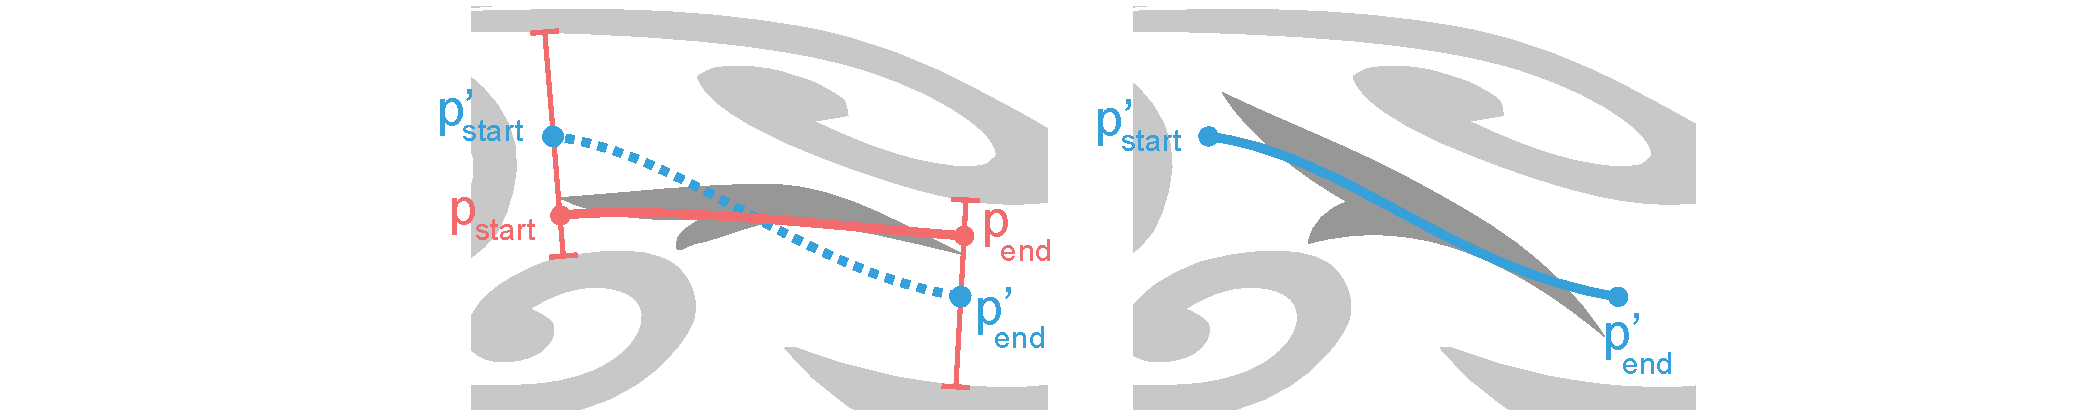
\includegraphics[width=6.4cm]{figures/flowpak/shift_streamline.pdf}
 \caption{\label{shift_streamline}
 Streamline shifting.
 	We move the streamline's start and end points along 
	perpendiculars, stopping before intersecting neighbouring elements.}
\smallskip

\includegraphics[width=3.2cm]{figures/flowpak/dijkstra.pdf}
 \caption{\label{dijkstra}
 Tracing a shortest path using Dijkstra's algorithm.  We generate the 
 orange nodes by resampling and offsetting the original red streamline.
          The search directions at a node are shown with green arrows.}
\end{figure}

Once we have chosen an element, we place it along the streamline using a
simple skeletal stroke algorithm~\cite{Hsu93}. We uniformly scale the element's width
to make it as wide as possible while still staying inside the blob
(Figure~\ref{shape_deformation}).

%%%%%%%%%%%%%%%%%%%%%%%%%%%%%%%%%%%%%%%%%%%%%%%%%%%%%%%%%%
\subsection{Iterative Refinement}
%%%%%%%%%%%%%%%%%%%%%%%%%%%%%%%%%%%%%%%%%%%%%%%%%%%%%%%%%%

\begin{figure}[t]
\centering

\includegraphics[width=6.5cm]{figures/flowpak/stretch.pdf}
\caption{\label{stretch_ornament}
(a) An elementt with its sub-region blob shown in dashed green line. Note that any blob is constrained by the neighboring elements. (b) The dashed red line is the grown blob, which accommodates an enlarged element.}

% ROTATING OR FLIPPING
\medskip
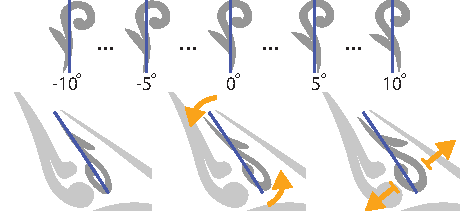
\includegraphics[width=6.5cm]{figures/flowpak/rotate_ornament.pdf}
\caption{\label{rotate_ornament}
Top row: rotated versions of the original element. 
         The best rotation angle is chosen via least squares matching.
         Bottom row: original, rotated, and enlarged versions of an element.}

\medskip
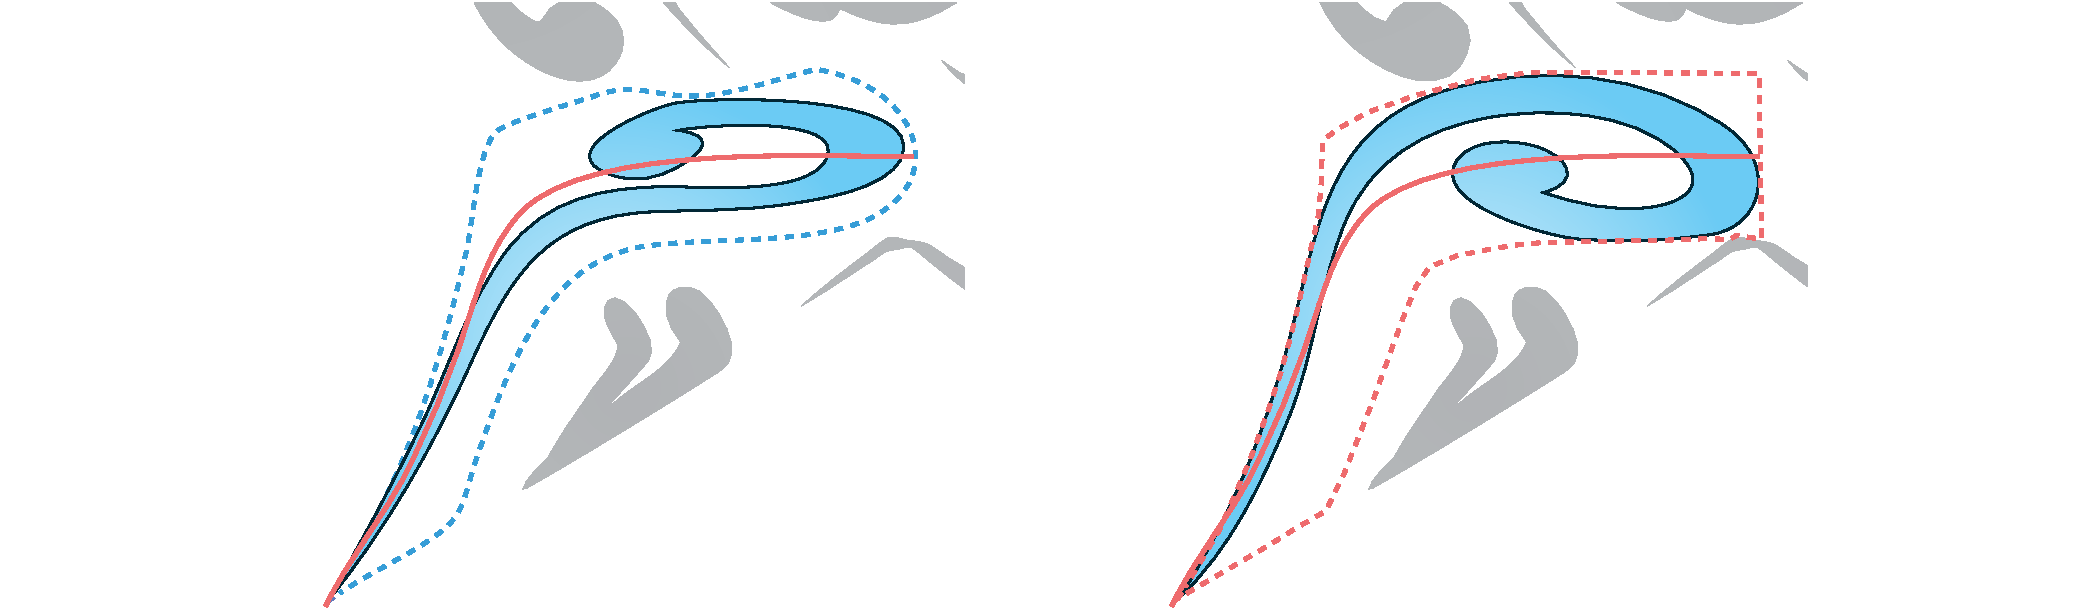
\includegraphics[width=4.5cm]{figures/flowpak/flip.pdf}
\caption{\label{flip_shape}
An element that reflects across its spine during iterative refinement.
LR functions and least squares shape matching allow an element to reflect
across its spine, along its spine, or both.}
\end{figure}

%%%%%%%%%%%%%%%%%%%%%%%%%%%%%%%%%%%%%%%%%%%%%%%%%%%%%%%%%%
\section{Implementation and Results}
%%%%%%%%%%%%%%%%%%%%%%%%%%%%%%%%%%%%%%%%%%%%%%%%%%%%%%%%%%

\begin{figure}
\centering
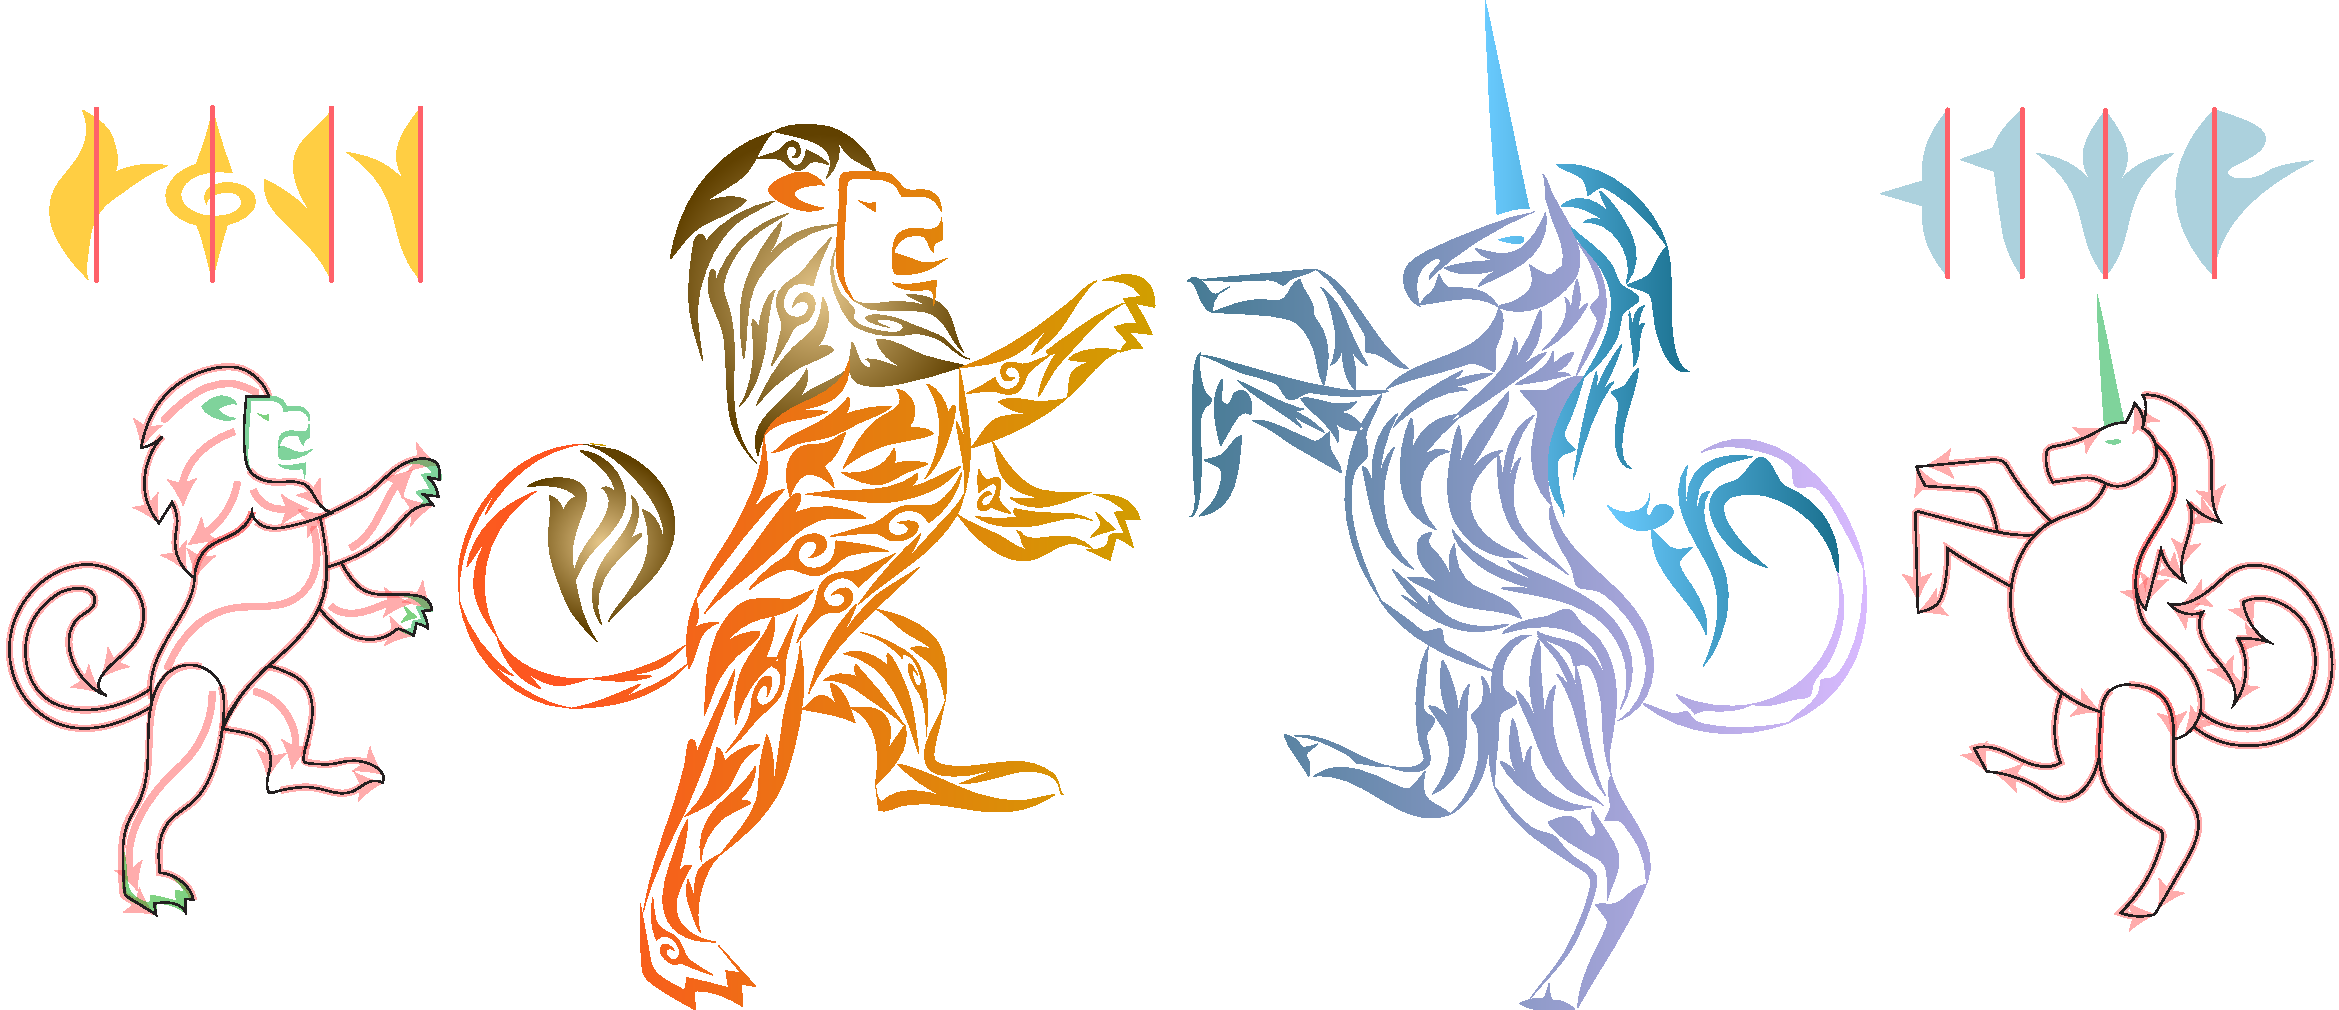
\includegraphics[width=1.0\textwidth]{figures/flowpak/lion_unicorn.pdf} 
\caption{\label{fig_lion_unicorn} 
Lion Unicorn. }
\end{figure}

\begin{figure}[t!]
\centering
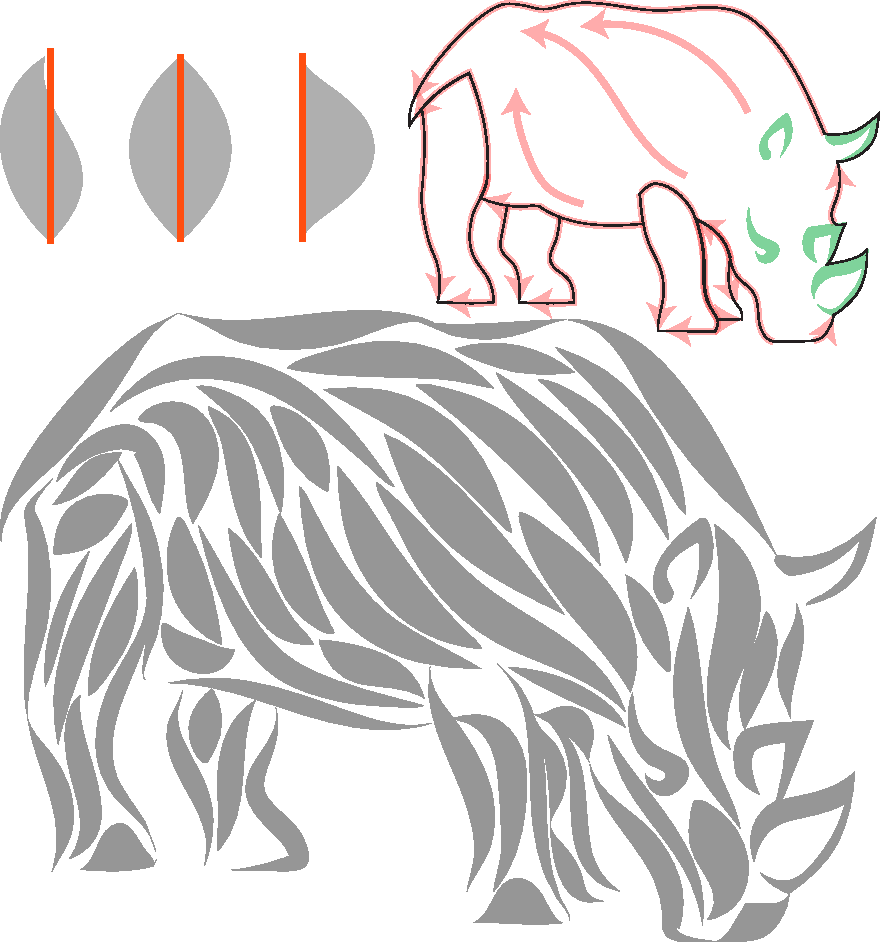
\includegraphics[width=5cm]{figures/flowpak/result_02.pdf} %RHINO
\caption{\label{result_rhino}
A packing of a rhinoceros.  Simple teardrop-shaped 
elements lead to variety in size and curvature.}
\bigskip
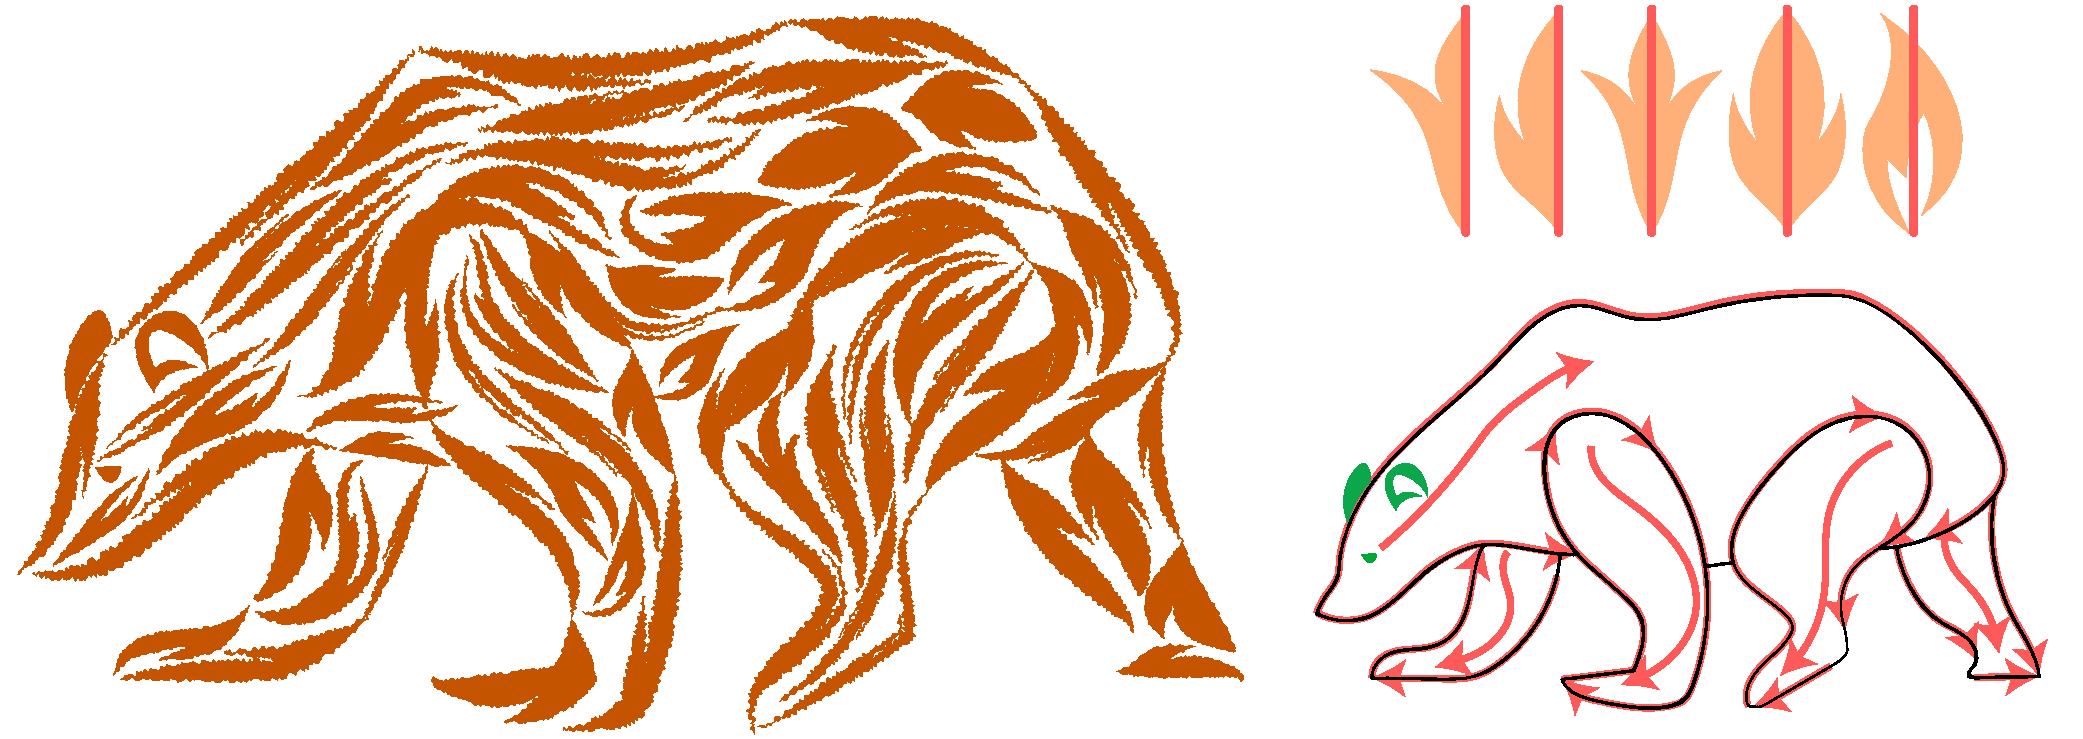
\includegraphics[width=6cm]{figures/flowpak/bear_leaves.pdf} %BEAR LEAVES
\caption{\label{result_bear_leaves}
	A bear packed with leaf elements.  We manually add noise to the 
	elements in the output to create a distressed look.}
\end{figure}

\begin{figure} %CAT
\centering
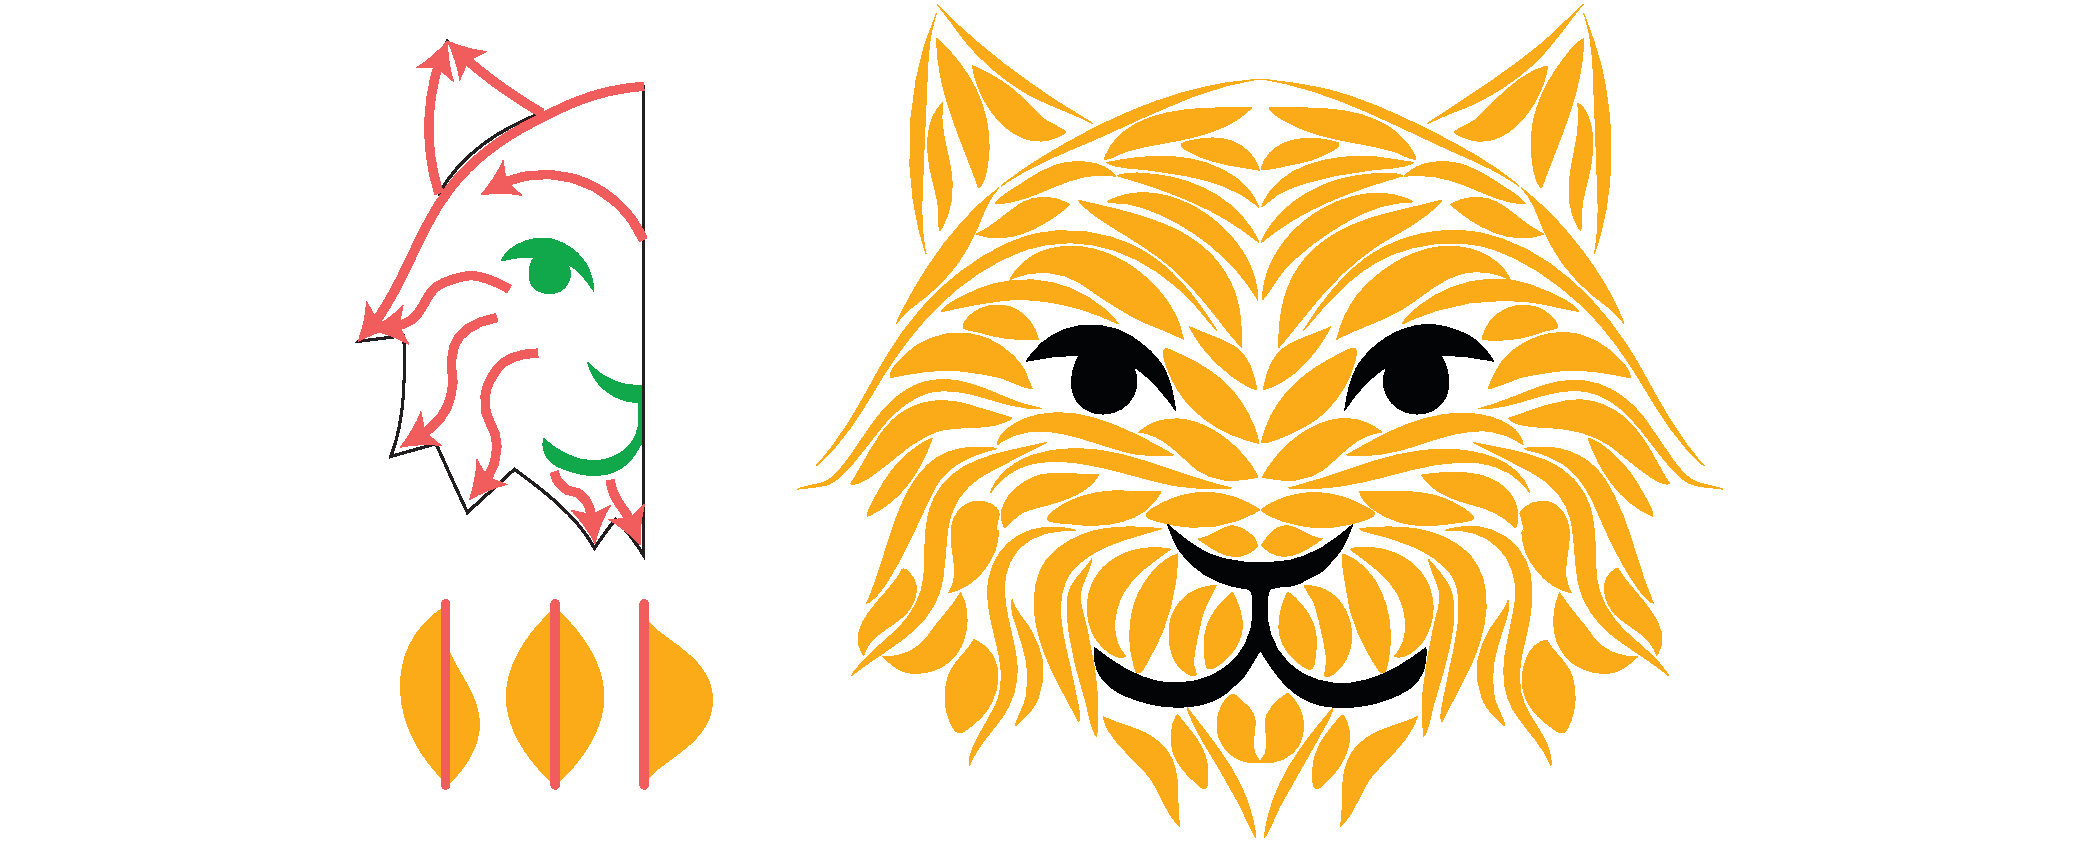
\includegraphics[width=6.5cm]{figures/flowpak/cat.pdf}
\caption{A packing with a symmetric layout; we only compute the left half and reflect the result. The elements around the cheeks and the chin are not aligned to the boundary, creating a fur-like effect.}
\label{result_cat}
\end{figure}


\begin{figure} %DOG FLOWER
\centering
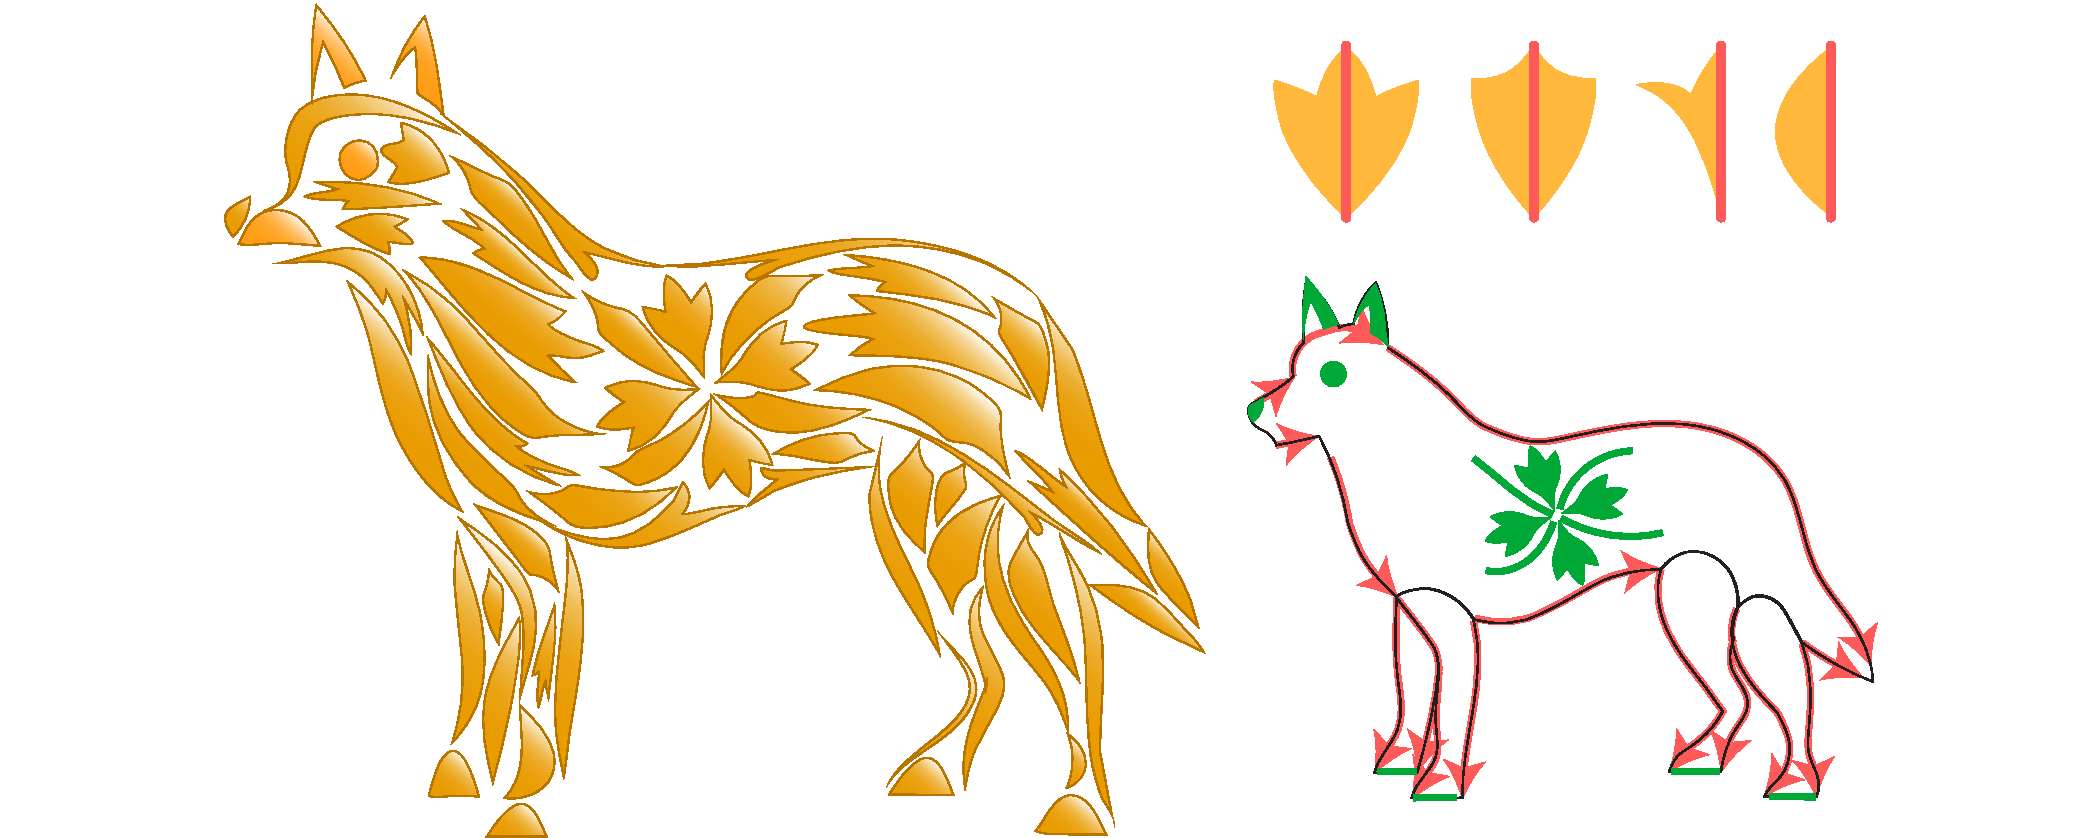
\includegraphics[width=6cm]{figures/flowpak/dog_flower.pdf}
\caption{A packing of a dog. The fixed elements, shown as green
	shapes in the diagram, are copied as-is to the output; fixed spines,
	shown as green paths, force the placement of new elements at the given
	locations.}
\label{result_dog}
\end{figure}




\begin{figure} %BEAR OFFSET
\centering
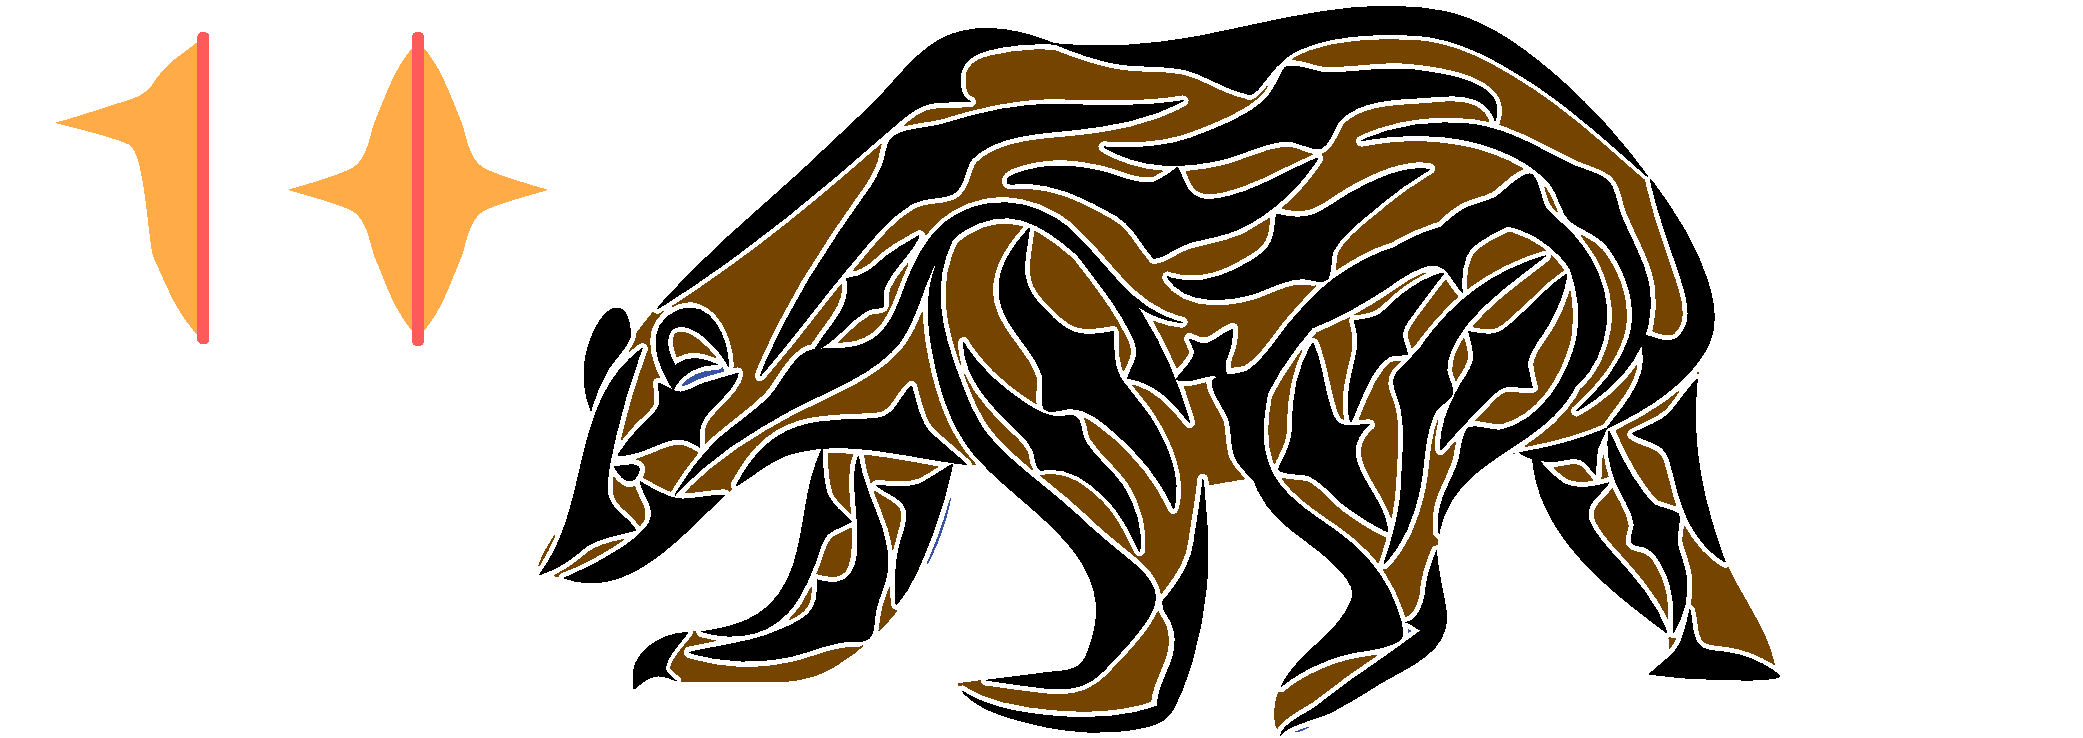
\includegraphics[width=6cm]{figures/flowpak/bear_offset_space.pdf}
\caption{A packing of the same container as in Figure~\ref{result_bear_leaves}.
	We place longer and sparser elements and synthesize additional forms to
	fill negative space.}
\label{result_bear_offset}
\end{figure}

\begin{figure} %BIRD SQUARE
\centering
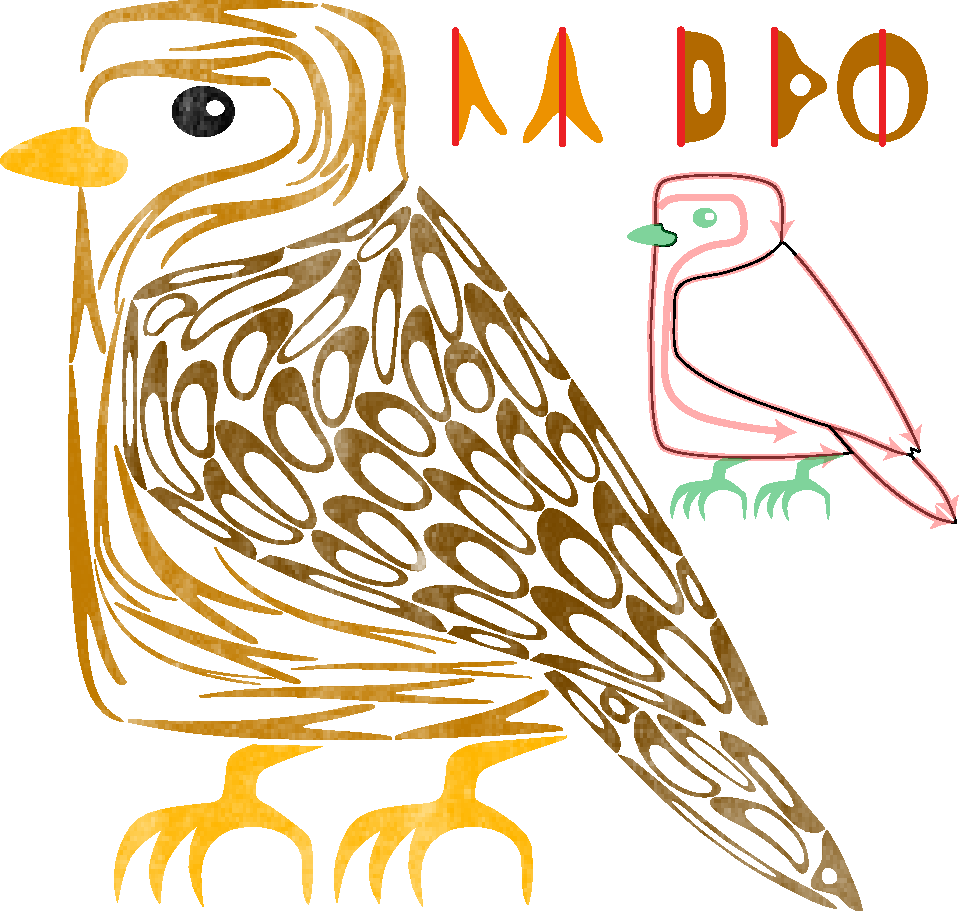
\includegraphics[width=6cm]{figures/flowpak/bird_square.pdf}
\caption{A packing of a bird, based on input provided by
	an artist.}
\label{bird_square}
\end{figure}

%%%%%%%%%%%%%%%%%%%%%%%%%%%%%%%%%%%%%%%%%%%%%%%%%%%%%%%%%%
\section{Conclusions}
%%%%%%%%%%%%%%%%%%%%%%%%%%%%%%%%%%%%%%%%%%%%%%%%%%%%%%%%%%

